\chapter{Design}\label{ch:design}

This chapter outlines the system's design, detailing its components in accordance with the requirements specified in \cref{ch:requirements}. The system consists of four core components: the \gls{uav}, responsible for providing the functionality and mobility, the control station, responsible for monitoring the \gls{uav} in real-time and updating its flight plan, the communication system, responsible for enabling real-time data exchange between the \gls{uav}, control station, and reconnaissance platform, and the reconnaissance platform, responsible for processing the data collected by the \gls{uav} and providing insights to the end-user. The full cost breakdown of the system is detailed in \cref{sec:budget_analysis}.

\todo{add schematic of the system}

\section{Unmanned Aerial Vehicle}\label{sec:design_uav}

For the \gls{uav} design, the following components are considered: the airframe, the propulsion system, the flight controller, the power system, and peripherals.

\subsection{Airframe}

The airframe is the structure of the \gls{uav} that holds all the components together. The airframe must be lightweight, durable, and easy to assemble and disassemble. The airframe must also be able to carry the peripherals and additional components required for the reconnaissance tasks.

For the airframe, different designes are considered, such as fixed-wing, rotary-wing, and hybrid designs as stated in \cref{sec:uav_types}. As on of the main requirements is the ability to take off and land in remote areas with limited infrastructure, a rotary-wing design is chosen for the \gls{uav}. The rotary-wing design allows for vertical takeoff and landing, as well as the ability to hover in place, which is useful for reconnaissance tasks.

Rotary-wing designs are further divided into multi-rotor and single-rotor designs as seen in \cref{fig:rotary_wing_designs}. Multi-rotor designs are more stable and easier to control, while single-rotor designs are more efficient and have a longer flight time. For the \gls{uav} design, a quadcopter design is chosen, as it provides a good balance between stability and efficiency.

\begin{figure}
  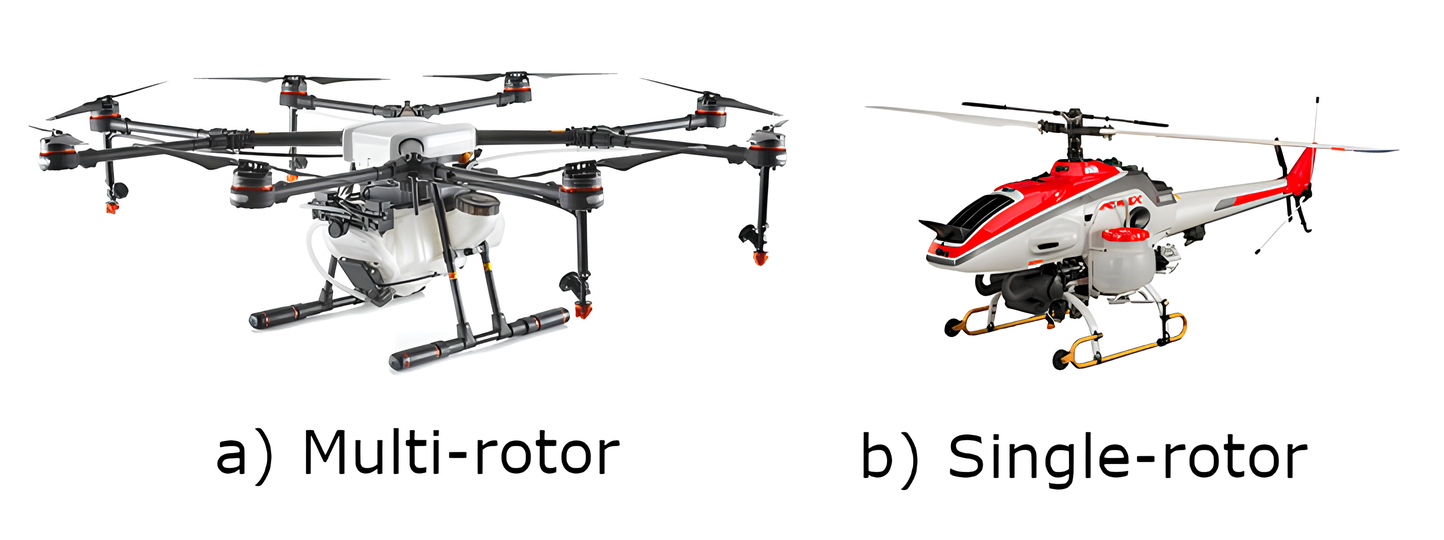
\includegraphics{rotary_wing_designs.png}
  \caption{Rotary-wing designs. Reproduced from \autocite{rotary_wing_designs}.
  }\label{fig:rotary_wing_designs}
\end{figure}

For the material of the airframe, a lightweight and durable material is chosen, such as carbon fiber or aluminum. The airframe is designed to be modular, allowing for the integration of different sensors and payloads for different applications. And finally, the airframe is designed to be cost-effective and commercially available, with the ability to be assembled and disassembled easily, and to be repaired and maintained with minimal effort.


For that case the airframe chosen \todo{add ref to where we bought it} is the \todo{add which one}. It is a quadcopter design made of carbon fiber, with a wingspan of \todo{add size} and a maximum takeoff weight of \todo{add weight}. The airframe is designed to carry a maximum payload weight of \todo{add weight}, with the ability to adapt to different reconnaissance tasks. Moreover, it has a payload bay that allows for the integration of different sensors and payloads, such as cameras, lidar, and thermal imaging sensors.

\todo{ add image of the aireframe chosen }

\subsection{Propulsion System}\label{subsec:design_propulsion_system}

The propulsion system is the system that provides the thrust required for the \gls{uav} to take off, land, and navigate. The propulsion system can be of different types, such as electric, gasoline, or hybrid. Electric propulsion systems are usually chosen for \glspl{uav} due to their efficiency, reliability, and low maintenance requirements. Gasoline propulsion systems are usually chosen for larger \glspl{uav} that require longer flight times and higher payloads. Hybrid propulsion systems are usually chosen for \glspl{uav} that require both efficiency and long flight times.

For the \gls{uav} design, an electric propulsion system is chosen, as it provides a good balance between efficiency, reliability, and low maintenance requirements. The electric propulsion system consists of four brushless motors, four electronic speed controllers, and four propellers. The main requirements of the propulsion system are the ability to provide enough thrust for the \gls{uav} to take off, land, and navigate, as well as the ability to carry the maximum payload weight of \todo{add weight}.

The brushless motors chosen were the \todo{add ref to where we bought them}, with a maximum thrust of \todo{add thrust} and a maximum power of \todo{add power}. The electronic speed controllers chosen were the \todo{add ref to where we bought them}, with a maximum current of \todo{add current} and a maximum voltage of \todo{add voltage}. The propellers chosen were the \todo{add ref to where we bought them}, with a maximum diameter of \todo{add diameter} and a maximum pitch of \todo{add pitch}. This complete propulsion system is designed to provide a thrust-to-weight ratio of \todo{add ratio}, with the ability to carry the maximum payload weight of \todo{add weight} which meets the requirements of the \gls{uav} design.

\todo{ add image of the propulsion system chosen }

\subsection{Flight Controller}

The flight controller is the system that controls the \gls{uav} during flight. The flight controller is responsible for stabilizing the \gls{uav}, controlling the motors, and navigating the \gls{uav} to a set of waypoints. The flight controller can be of different types, such as manual, semi-autonomous, or autonomous. Manual flight controllers are usually chosen for \glspl{uav} that require human intervention during flight. Semi-autonomous flight controllers are usually chosen for \glspl{uav} that require human intervention for takeoff and landing, but can navigate autonomously to a set of waypoints. Autonomous flight controllers are usually chosen for \glspl{uav} that can take off, land, and navigate autonomously to a set of waypoints. One key feature of the flight controller is the \textit{Return to Home} feature, which allows the \gls{uav} to return to the ground station in case of loss of communication or other critical failures.

For the \gls{uav} design, an autonomous flight controller is chosen, as it provides the ability to take off, land, and navigate autonomously to a set of waypoints. Commercially, there are multiple flight controllers available \todo{ref to table} and any of them can be used for the \gls{uav} design. The main requirements of the flight controller are the ability to stabilize the \gls{uav}, control the motors, and navigate the \gls{uav} to a set of waypoints, as well as the ability to communicate with the ground station in real-time. The flight controller chosen was the \todo{add ref to where we bought it}, as \todo{add reasons} An image of the flight controller is shown in \todo{add ref to fig}.

\todo{ add table of flight controllers }

\todo{ add image of the flight controller chosen }

\subsection{Power System}\label{subsec:design_power_system}

The power system is the system that provides the power required for the \gls{uav} to operate. The power system can be of different types, such as batteries, fuel cells, or solar panels. For \glspl{uav}, usually batteries are chosen, as they provide a good balance between energy density, power density, and weight. The main requirements of the power system are the ability to provide enough power for the \gls{uav} to take off, land, and navigate, as well as the ability to carry the maximum payload weight of \todo{add weight}.

For the \gls{uav} design, a lithium polymer battery is chosen, as it provides a good balance between energy density, power density, and weight. The battery chosen was the \todo{add ref to where we bought it}, with a maximum capacity of \todo{add capacity} and a maximum voltage of \todo{add voltage}. The battery is designed to provide enough power for the \gls{uav} to take off, land, and navigate, as well as the ability to carry the maximum payload weight of \todo{add weight}. The battery is also designed to be modular, allowing for the integration of different batteries for different applications.

\todo{ add image of the power system chosen }

Moreover, usually the power system is divided into two parts, the power distribution system for the propulsion system and the power management system for the electronics. The main reason for this distinction is that the propulsion system requires a high current and low voltage, while the electronics require a low current and high voltage. However, for the \gls{uav} design, the power system is integrated into a single system to reduce weight and complexity and specially the pricing of the system.

Futhermore, in order to provide the required power for the different components of the \gls{uav}, a power management system is integrated into the power system. The power management system consists of a battery monitor, a voltage regulator, and a current sensor. The one chosen was the \todo{add ref to where we bought it}, with a maximum current of \todo{add current} and a maximum voltage of \todo{add voltage}. The power management system is designed to provide the required power for the different components of the \gls{uav}, as well as the ability to monitor the battery voltage and current in real-time. And finally, a voltage regulator is integrated into the power system to provide the required voltage for the reconnaissance platform and the communication system. The voltage regulator chosen was the \todo{add ref to where we bought it}, with a maximum voltage of \todo{add voltage} and a maximum current of \todo{add current}. The voltage regulator is designed to provide the required voltage for the reconnaissance platform and the communication system, as well as the ability to monitor the voltage and current in real-time.

\todo{ add image of the power management system chosen }

\subsection{Peripherals}

The peripherals are the components that provide additional functionality to the \gls{uav}. The peripherals can be of different types, such as sensors, geo-location systems, cameras, lidar, or thermal imaging sensors. For reconnaissance tasks, usually cameras are chosen, as they provide the ability to collect images of the environment. But other sensors can be integrated into the \gls{uav} to provide additional functionality, such as geo-location systems for navigation, lidar for obstacle avoidance, or thermal imaging sensors for monitoring the environment.

For the \gls{uav} design, a \gls{gps} module was integrated into the \gls{uav}, as it provides the ability to navigate the \gls{uav} to a set of waypoints. The \gls{gps} module chosen was the \todo{add ref to where we bought it}, with a maximum accuracy of \todo{add accuracy} and a maximum update rate of \todo{add rate}. The \gls{gps} module is designed to provide the ability to navigate the \gls{uav} to a set of waypoints, as well as the ability to relay the information to the ground station in real-time. An image of the \gls{gps} module is shown in \todo{add ref to fig}.

\todo{ add image of the gps module chosen }

Moreover, a kill switch was integrated into the \gls{uav}, as it provides the ability to stop the motors in case of an emergency. It is a required safety feature for \glspl{uav} to prevent accidents and injuries. The kill switch chosen was the \todo{add ref to where we bought it}.

\todo{ add image of the kill switch chosen }

Finally, a camera was integrated into the \gls{uav}, as it provides the ability to collect images of the environment. The camera chosen was the \todo{add ref to where we bought it}, with a maximum resolution of \todo{add resolution} and a maximum frame rate of \todo{add rate}. The camera is designed to provide the ability to collect images of the environment, as well as the ability to relay the information to the ground station in real-time. An image of the camera is shown in \todo{add ref to fig}.

\todo{ add image of the camera chosen }

% Local Variables:
% jinx-local-words: "aireframe uav"
% End:

\section{Control Station}\label{sec:design_control_station}

The control station is the station that monitors the \gls{uav} in real-time. It is responsible for receiving telemetry data from the \gls{uav} and sending commands to update its flight plan. The control station is also responsible for creating a geofence around the area of operation, monitoring the \gls{uav}'s position and altitude in real-time, and tracking multiple \glspl{uav} simultaneously. To perform the tasks mentioned, the control station is composed of a ground control station running a waypoint planning software and a radio controller with a communication module to communicate with the \gls{uav} in real-time.

The ground control station is the human-machine interface that allows the operator to monitor the \gls{uav} in real-time, receive telemetry data from the \gls{uav}, and send commands to update its flight plan. For the ground control station, a personal laptop or a desktop computer is used with the waypoint planning software installed, in this case, the Mission Planner software \autocite{ardupilotMissionPlanner}. For the radio controller, a handheld device is used that allows the operator to take control of the \gls{uav} manually in case of an emergency and a communication module to receive telemetry data from the \gls{uav} in real-time. The radio controller used is the RadioMaster TX16S MKII Hall V4.0 \autocite{rcinnovationsRadioMasterTX16S}. For the communication module, the module used is described in \cref{sec:design_communication_system}.

% Local Variables:
% jinx-local-words: "ardupilotMissionPlanner uav"
% End:

\section{Reconnaissance Platform}\label{sec:design_reconnaissance_platform}

The reconnaissance platform is the system that processes the data collected by the peripherals and the sensors on the \gls{uav} and provides insights to the end-user for the different reconnaissance tasks. The reconnaissance platform is responsible detecting and tracking objects, monitoring the environment, and generating alerts and notifications in case of critical events or failures. The reconnaissance platform is also responsible for coordinating the flight plans of the \glspl{uav} in a swarm, as well as designing the missions for the \glspl{uav} to perform specific tasks.

The reconnaissance platform is divided into two main components depending on where they run, the on-board reconnaissance platform and the off-board reconnaissance platform.

\subsection{On-Board Reconnaissance Platform}\label{subsec:on-board_reconnaissance_platform}

The on-board reconnaissance platform is the system that runs on the \gls{uav} and is responsible for processing the data collected by the \gls{uav} and providing insights to the end-user. The on-board reconnaissance platform is composed of a on-board computer and a communication module to communicate with the off-board reconnaissance platform.

For the on-board computer, multiple options were considered as represented in \todo{add table reference}. The main use case for the reconnaissance platform is to process the data collected by the \gls{uav} in real-time and provide insights to the end-user. For this case, a computer with a high processing power, specially in the \gls{gpu}, is required as deep learning algorithms are used to detect and track objects in the environment. The on-board computer chosen for the reconnaissance platform was the \todo{add ref to where we bought them} depicted in \todo{add figure}, as it provides a good balance between processing power, reliability, and price-performance ratio. The reason to choose this on-board computer is that it provides the highest processing power commercially available. Having a stable and reliable on-board computer is crucial for the \gls{uav} design, as it allows for the \gls{uav} to process the data collected in real-time and provide insights to the end-user. Moreover, it is widely used in the industry and has a large community of developers, which makes it easier to find support and documentation.

\todo{add table with the on-board computer options}

\todo{add figure of the on-board computer}

For the communication module, a \gls{4g} communication module was chosen, as it provides a high bandwidth required to send the data collected by the \gls{uav} in real-time to the off-board reconnaissance platform and a simple yet robust communication system. The communication module chosen for the on-board reconnaissance platform was the \todo{add ref to where we bought them} depicted in \todo{add figure}, as it provides a good balance between bandwidth, reliability, and price-performance ratio. For the use case of this project, a \gls{4g} communication module was enough as the environment where the \gls{uav} will operate has a good \gls{4g} coverage. On the other hand, if the \gls{uav} will operate in remote areas with limited infrastructure, a \gls{rf} communication module would be more suitable.

\todo{add figure of the communication module}

\todo{also add a camera}

\subsection{Off-Board Reconnaissance Platform}\label{subsec:off-board_reconnaissance_platform}

The off-board reconnaissance platform is the system that runs on a server and is responsible for coordinating the missions of the \glspl{uav} in a swarm, as well as generating reports and analyzing the data collected by the \glspl{uav}. The off-board reconnaissance platform is composed of a server, a database, and a communication module to communicate with the on-board reconnaissance platform.

For the server, multiple options were considered as represented in \todo{add table reference}. The main use case for the reconnaissance platform is to process the data collected by the \glspl{uav} in real-time and provide insights to the end-user. For this case, a server with a stable and reliable connection is required. Moreover, the server should be able to be accessed remotely from anywhere in the world, as the end-user may be located in a different location than the server. For this the option that was chosen was the \todo{add ref to where we bought them} as it provides the best price-ease of use ratio. The reason to choose a cloud provider is that it provides a stable and reliable connection, as well as the ability to be accessed remotely from anywhere in the world. Moreover, it is widely used in the industry and has a large community of developers, which makes it easier to find support and documentation.

\todo{add table with the server options}

\section{Communication System}\label{sec:communication_system}

The communication system is the system that allows the \gls{uav} to communicate with the ground station in real-time, as well as providing the connection to the reconnaissance platform. The communication system is responsible for sending telemetry data from the \gls{uav} to the ground station, receiving commands from the ground station to update the \gls{uav}'s flight plan, and sending the data collected by the \gls{uav} to the reconnaissance platform for further analysis. Different communication systems can be used depending on the use case, such as \gls{4g}, \gls{3g}, \gls{wifi}, or \gls{rf}, and the environment where the \gls{uav} will operate. The characteristics to consider when choosing a communication system can be seen in \todo{add ref to the table in the requirements chapter}.

\todo{add table with the communication system options}

For this project, two comunication systems were chosen the on-board communication system and the off-board communication system.

\subsection{On-Board Communication System}\label{subsec:on-board_communication_system}

The on-board communication system is the system that connects the \gls{uav} with the ground station in real-time. The on-board communication system is composed of a communication module that sends telemetry data from the \gls{uav} to the ground station and receives commands from the ground station to update the \gls{uav}'s flight plan. The on-board communication system is responsible for providing a stable and reliable connection between the \gls{uav} and the ground station, as well as a high bandwidth to send the data collected by the \gls{uav} to the reconnaissance platform. The main requirements for the on-board communication system are a high reliability, a low latency, and long range.

For this case, a \gls{rf} communication module was chosen, as it satisfies the requirements for the on-board communication system as well as not needing a cellular network to operate, thus making it more versatile and ideal to operate in remote areas. The \gls{rf} communication module chosen for the on-board communication system was the \todo{add ref to where we bought them} depicted in \todo{add figure}, as it provides a good balance between reliability, latency, and range. The reason to choose a \gls{rf} communication module is that it provides a stable and reliable connection, as well as a low latency and long range. Moreover, it is the defacto standard for \gls{uav} communication systems, as it provides a good price-performance ratio.

\todo{add figure of the communication module}

\subsection{Off-Board Communication System}\label{subsec:off-board_communication_system}

The off-board communication system is the system that connects the on-board reconnaissance platform with the off-board reconnaissance platform. The off-board communication system is composed of a communication module that sends the data collected by the \gls{uav} to the off-board reconnaissance platform for further analysis. The off-board communication system is responsible for providing a stable and reliable connection between the on-board reconnaissance platform and the off-board reconnaissance platform, as well as a high bandwidth to send the data collected by the \gls{uav} in real-time. The main requirements for the off-board communication system are a high bandwidth, a secure connection, and the ability to receive data from multiple \glspl{uav} simultaneously.

For this case, a \gls{4g} communication module was chosen, as it satisfies the requirements for the off-board communication system as well as providing a high bandwidth to send the data collected by the \gls{uav} in real-time. The \gls{4g} communication module chosen for the off-board communication system was the \todo{add ref to where we bought them} depicted in \todo{add figure}, as it provides a good balance between bandwidth, reliability, and price-performance ratio. A \gls{4g} communication module was chosen as the environment where the \gls{uav} will operate has a good \gls{4g} coverage. On the other hand, if the \gls{uav} will operate in remote areas with limited infrastructure, a \gls{rf} communication module would be more suitable.

\todo{add figure of the communication module}


% Local Variables:
% jinx-local-words: "uav"
% End:
